\documentclass[tikz]{standalone}
\usepackage{amsmath}
\usepackage{tikz}

\begin{document}
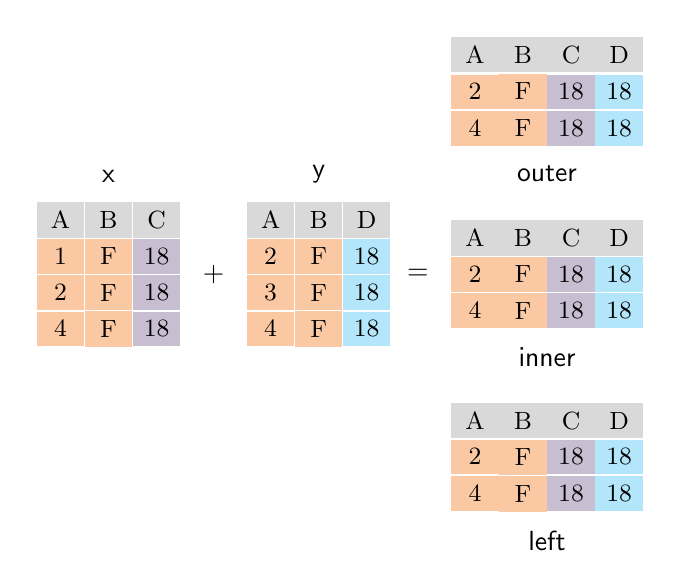
\begin{tikzpicture}[font=\sffamily ,
varName/.style={rectangle, fill=gray!30, minimum height=0.4cm, minimum width=0.6cm, font=\small} ,
varValue/.style={varName, fill=yellow!30!red!30} ,
sep/.style={row sep=0.1mm, column sep=0.1mm} ,
C/.style={fill=yellow!30!blue!30} ,
D/.style={fill=cyan!30}
]
\node (plus) {+} ;

\matrix (X) at (plus) [left=0.3cm, label=above:x, sep] {
    \node [varName] {A} ; & \node [varName] {B} ; & \node [varName] {C} ; \\
    \node [varValue] {1} ; & \node [varValue] {F} ; & \node [varValue, C] {18} ; \\
    \node [varValue] {2} ; & \node [varValue] {F} ; & \node [varValue, C] {18} ; \\
    \node [varValue] {4} ; & \node [varValue] {F} ; & \node [varValue, C] {18} ; \\
} ;
\matrix (Y) at (plus) [right=0.3cm, label=above:y, sep] {
    \node [varName] {A} ; & \node [varName] {B} ; & \node [varName] {D} ; \\
    \node [varValue] {2} ; & \node [varValue] {F} ; & \node [varValue, D] {18} ; \\
    \node [varValue] {3} ; & \node [varValue] {F} ; & \node [varValue, D] {18} ; \\
    \node [varValue] {4} ; & \node [varValue] {F} ; & \node [varValue, D] {18} ; \\
} ;

\node (equal) at (Y) [right=1.0cm] {=} ;

\matrix (inner-join) at (equal) [right=0.3cm, label=below:inner, sep] {
    \node [varName] {A} ; & \node [varName] {B} ; & \node [varName] {C} ; & \node [varName] {D} ; \\
    \node [varValue] {2} ; & \node [varValue] {F} ; & \node [varValue, fill=yellow!30!blue!30] {18} ; & \node [varValue, D] {18} ; \\
    \node [varValue] {4} ; & \node [varValue] {F} ; & \node [varValue, fill=yellow!30!blue!30] {18} ; & \node [varValue, D] {18} ; \\
} ;

\matrix (outer-join) at (inner-join) [above=1.5cm, label=below:outer, sep] {
    \node [varName] {A} ; & \node [varName] {B} ; & \node [varName] {C} ; & \node [varName] {D} ; \\
    \node [varValue] {2} ; & \node [varValue] {F} ; & \node [varValue, fill=yellow!30!blue!30] {18} ; & \node [varValue, D] {18} ; \\
    \node [varValue] {4} ; & \node [varValue] {F} ; & \node [varValue, fill=yellow!30!blue!30] {18} ; & \node [varValue, D] {18} ; \\
} ;

\matrix (left-join) at (inner-join) [below=1.5cm, label=below:left, sep] {
    \node [varName] {A} ; & \node [varName] {B} ; & \node [varName] {C} ; & \node [varName] {D} ; \\
    \node [varValue] {2} ; & \node [varValue] {F} ; & \node [varValue, fill=yellow!30!blue!30] {18} ; & \node [varValue, D] {18} ; \\
    \node [varValue] {4} ; & \node [varValue] {F} ; & \node [varValue, fill=yellow!30!blue!30] {18} ; & \node [varValue, D] {18} ; \\
} ;
\end{tikzpicture}

\end{document}
